\documentclass[a4paper,notitlepage]{article}
\usepackage{pfsstyle}

\title{\[DRAFT\] Instrument Control Software interface design document \\
    plan C proposal}
\author{Atsushi Shimono (PFS Software Team)}
\begin{document}

\maketitle
\tableofcontents

\section{Abstract}

For an architectural design of the ICS (Instrument Control Software), 
we have two proposals: instrument architecture with the super subsystem 
to control everything related with the positioner control, and software 
design with one central messaging hub to connect every controllable 
subsystems. 
In this design document, an alternate software architectural design for 
the PFS is described, which takes advantages from both plans. 
As PFS science requirement, the instrument control software should work 
in collaboration with the targeting software and the on-site data 
reduction pipeline, this document does not touch these interfaces in 
detail.

Also to prevent future confusions and misunderstandings, 
this design document proposes definitions of naming, terminology, and 
their covering area, independently from wording at the Subaru.


\section{Background of software designs}

Entire instrument control software will be derivered and work at the 
Subaru Summit Facility (SSF) in cooperation with the Subaru telescope 
control systems.

\subsection{Relation to the Subaru telescope}

In the Subaru telescope control systems (so called SOSS), (whole) instrument 
control system are called as OBCP
\footnote{What OBCP stands of is not clear, and also its definition varies 
by sentences.} but its naming and role are not clear from instrument 
control point of view.
Here, we define interfaces of our PFS instrument control system to the 
Subaru telescope control system as followings.

\begin{description}
  \item[ICS] Instrument Control System, which includes everything of the 
    PFS instrument control software systems including every subsystem 
    control software. ICS will include any required engineering software 
    including graphical user interfaces, command-line user interfaces, or 
    network data API, but will not include any connected systems at the SSF 
    such as an on-site data reduction pipeline or a targeting software 
    instance. 
  \item[IIC] Instrument Interface and Controller, which has two roles: 
    the only interface of the ICS to the Subaru telescope control system 
    including Gen2, TCS, MLP1 and any other possible candidates; the master 
    controller and sequencer for the entire ICS.
  \item[MHS] Messaging Hub Server, which is the only central communication hub 
    system in entire ICS and every controllable subsystems and environment 
    monitoring systems will connect to this communication hub for sending or 
    recieving commands to peers, sharing status messages, arising operational 
    or environmental alerts, etc.
\end{description}

Normally, from the Subaru telescope (or SOSS) side, ICS or IIC will be visible 
as so called 'OBCP'. Also, except for some required direct connections to MLP, 
this ICS or IIC will the only peer from the PFS instrument control software. 


\subsubsection{Communication paths between ICS and SOSS}

To work in coordinate with the Subaru telescope, IIC should have connections 
to the SOSS by standard procedures defined by the Subaru telescope. 
These procedures and connections are summarized in 
Figure.~\ref{fig:ics-soss-connection}. 

\begin{figure}[htb]
  \begin{center}
    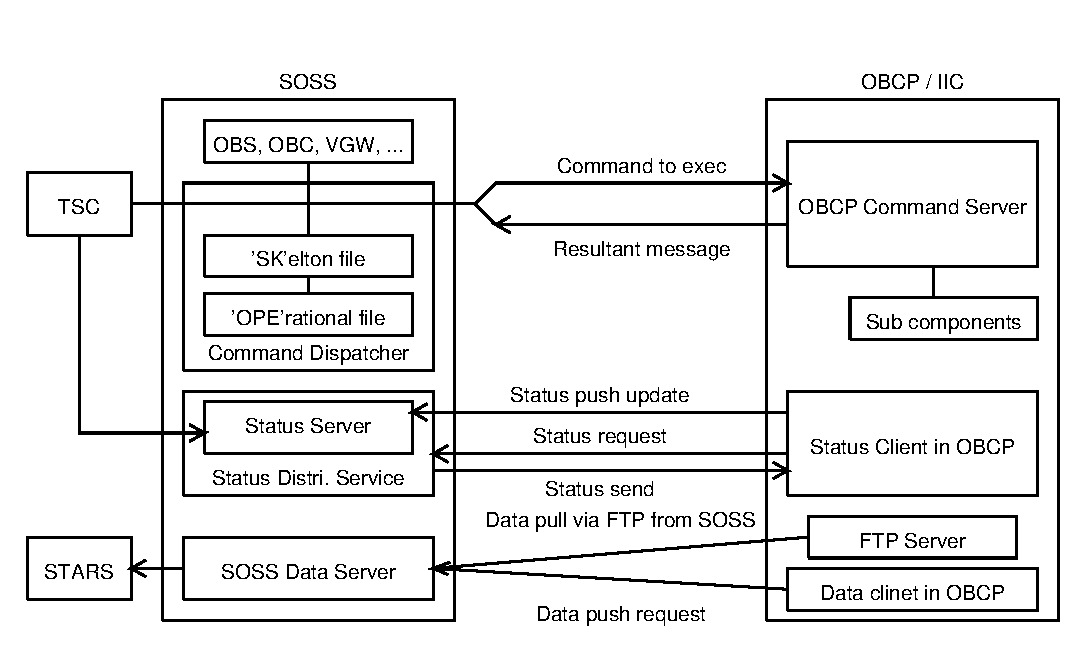
\includegraphics[scale=0.75]{ics-soss-connection.eps}
  \end{center}
  \caption{Connections between SOSS and OBCP. Wordings are of SOSS, not of 
      defined in this document.}
  \label{fig:ics-soss-connection}
\end{figure}

Each connection between SOSS and OBCP means: 

\begin{description}
  \item[Command to exec] One line of text in a format of 'COMMAND NAME=VALUE 
    NAME=VALUE ....' to be executed by the instrument (or any other system 
    controllable from the command dispatcher, including TCS). 
  \item[Resultant message] Result of a command execution including success or 
    not, status message.
  \item[Status push update] Each instrument is required to push its own status 
    to the status server of SOSS when status was changed. This status update 
    is triggerd by the instrument side.
  \item[Status request] Each instrument can request to retrieve any status 
    stored in the SOSS status server at any time. Note, the status distriburion 
    service has a matrixed permission table with statuses from which instrument 
    could be sent to which instrument. 
  \item[Status send] The status distribution service will send stored status 
    by request. 
  \item[Data pull via FTP from SOSS] To archive observed or created data, 
    SOSS data server will access a FTP service in each instrument to get 
    a specified file. 
  \item[Data push request] Each instrument should submit a data push request 
    with a ID specified by SOSS and a file name accessible via FTP, when data 
    is ready to send and be archived. 
\end{description}

\subsubsection{Samples of current sk and ope files}

Since 'sk' and 'ope' files are used in the current SOSS (or Gen2), and we are 
planning to have another mechanism (or protocol), their file formats will not 
directly effect to our software design, but it is important to understand 
how commands will flow into the instrument. 
Both of sk and ope files are dispatched line by line, especially for ope file 
which will be selected by operator or observer line by line. 

Each line in ope files will be like : 

\begin{verbatim}
GETOBJECT EXPTIME=1800 $OBJECT $OBJECT_CONFIG $DEF_IMAG $IMPOS BINNING=3X3
GETBIAS $DEF_IMAG BINNING=3X3
MOVEGUIDE DELTA_RA=0.5 DELTA_DEC=-1.5 $DEF_TOOL
\end{verbatim}

and first word in each line will indicate which sk file to use. (Note, word 
starting with \$ means macro word, and will be translated into pre-defined 
set of words.) 
SOSS will read and execute commands written in each specified sk file, 
which is consisted with lines like :

\begin{verbatim}
Exec K3D WaitExp ;
Exec K3D ChPos MotorName=Mask PositionName=None ;
Exec OBS SetStatus Instrument_Name=K3D Object=$OBJECT ;
Exec OBC QDAS_Display Instrument_name=K3D Input_Frame=!STATOBS.K3D.C1 ;
Exec TSC AG_Tracking Motor=OFF Calc_Region=1 ;
Exec TSC AG Readout=OFF,
Exec VGW Mark_Position V_LAN_DATA=AG Mode=Clear ,
\end{verbatim}

Second word following 'Exec' indicates which instrument (or telescope, 
subsystems in SOSS; in above sample, K3D is the target instrument) 
to send command, and every words following instrument 
indicator will be directly sent to the instrument as a command line 
(including command parameter). Each command parameter is written in name=value 
format, values starting with \$ (operational or pre-defined parameter), or \! 
(SOSS internal working parameter, such as status) will be translated before 
sending to a specified instrument. 

\subsection{Role and capabilities of MHS --- Messaging Hub Server}
\label{MHS_Role}

MHS will be the only central messaging exchange system for entire PFS 
instrument including every controllable subsystems. 
To coordinate instrument control in a proper way, 
following requirements are applied to a selection of PFS MHS. 

\begin{itemize}
  \item MHS should be a star-liked message transfer and delivery system, 
    and does not require any (messy) multi-point to multi-point connection.
  \item MHS should have a capability per each peer to set / select 
    a list of acceptable peers, from which commands should be accepted and 
    otherwise should be rejected, as a configuration. 
    This could be implemented at the MHS side or at peers' side as a wrapper 
    layor; both could be accpetable.
  \item MHS should have a capability to attach external log servers as its 
    peers for every messages through the MHS. 
  \item MHS shuold have a capability to set a 'blocking flag' by each peer 
    to specify peers whose commands should be acceptable, on demand.
\end{itemize}

For a 'blocking flag', we need to be careful on the system deadlock, 
especially while defining interfaces. 

\subsection{Controllable subsystems and constraints}

Controllable subsystems within the PFS are: 

\begin{itemize}
  \item Detector control and readout systems (DCR) for CCDs and IR detectors
  \item Shutter mechanisms controller (SMC)
  \item Fiber back illuminating system (FIS)
  \item Acquisition and Guidance camera (AGC) system
  \item Prime Focus Instrument Control Software (PFICS)
  \item Metrology camera system (MCS)
\end{itemize}

Also, each subsystem should have an environment monitoring system (EMS) to 
measure environment statuses (such as temperatures, humidities, or 
illumination) and to send these statuses to EAD. 

Subsystems required for functionality of IIC and MHS are: 

\begin{itemize}
  \item Environment (Status) archive database (EAD) service
  \item Event logger database (ELD) service
\end{itemize}

Possible controllable subsystems within the PFS are: 

\begin{itemize}
  \item Slit viewing camera system (SVC)
  \item Slit position fine-adjustment system (SPF)
\end{itemize}

Controllable subsystems which could be under PFICS and may not be directly 
connected to MHS: 

\begin{itemize}
  \item Fiducial fiber back illuminating system (FFIS)
  \item COBRA Positioner Movement Planning Software (MPS)
\end{itemize}

\subsubsection{DCR --- Detector control and readout system}
\paragraph{Definition and subsystem hardware}
DCR will include every controllable hardware within dewar and detector systems, 
which will include detector movement (tilt?) mechanisms, cryostat vacuum and 
cooling system. 
\paragraph{Peers required to communicate}
DCR should receive commands from IIC, and should transfer retrieved data from 
detector subsystems to the data archive system (SOSS Data Server; STARS) of 
the Subaru telescope through IIC. 
\paragraph{Remarks}
Considering amount of controllable hardwares, this subsystem could be divided 
into two or more subsystems: detector control and any others. 

\subsubsection{SMC --- Shutter mechanisms controller}
\paragraph{Definition and subsystem hardware}
SMC will control shutter mechanisms (one per each spectrograph) to open or 
to close. 
\paragraph{Peers required to communicate}
SMC should receive commands from IIC. 
\paragraph{Remarks}
This shutter is a mechanism to: 
\begin{itemize}
  \item control an exposure time by shielding detectors from fiber outputs
  \item shield detectors from light source for fiber back illumination
  \item back illuminate science fibers by reflecting light with a diffuse 
    reflector mounted on shutter plate
\end{itemize}
Since this shutter is the only mechanism to shield detectors from fiber and 
light source for fiber back illuminator, SMC and its parent control system 
(assuming IIC) should control: 
\begin{itemize}
  \item OPEN during exposure
  \item CLOSE during detectors' reading out and light source illumination
\end{itemize}

\subsubsection{FIS --- Fiber back illuminating system}
\paragraph{Definition and subsystem hardware}
FIS will turn on/off and adjust brightness of back illuminating light source 
for science fibers. 
\paragraph{Peers required to communicate}
FIS should receive commands both from IIC and PFICS. 
\paragraph{Remarks}
Since back illuminating light source for science fibers should not be turned 
on while shutter is open (except for engineering or test purpose), IIC should 
coordinate to block control of FIS depending on a status of SMC. 

\subsubsection{AGC --- Acquisition and Guidance camera system}
\paragraph{Definition and subsystem hardware}
AGC should control Acquisition and Guidance camera system to meet 
requirements from procedures of both Acquisition and Auto 
Guiding. 
Also, for engineering, integration and testing purpose, AGC might need to work 
in cooporate with PFICS. 
\paragraph{Peers required to communicate}
AGC should receive commands from IIC, and should transfer measured guide 
signal (target field positioning error for Acquisition and Guidance per 
request, guider error for Auto Guiding in commanded rate) back to IIC. 
IIC should apply coordinate transformation and transfer to suitable peer, 
such as OCS or MLP1. 

(TBD) Also, if requested by an operator, 
AGC should transfer retrieved raw data image to a handling system (VGW). 
\paragraph{Remarks}
Especially for Auto Guiding feature, data transfer should work in strict 
timing. 
AGC might be required to connect and to work in cooporate with IIC in deeply. 

\subsubsection{PFICS --- Prime Focus Instrument Control Software}
\paragraph{Definition and subsystem hardware}
PFICS will also be a master controller for everything related with COBRA 
positioners, and this should work in close collaboration with MPS. 
Also, since this includes 'movement planning and sequencing', PFICS is 
required to issue commands to required subsystems for alignment of 
positioners, including turning on and off FIS, getting list of measured 
positions from MCS. 
\paragraph{Peers required to communicate}
PFICS should receive commands from IIC, and should send commands to all related 
external subsystems like MCS and FIS, and to all subsystems under this PFICS 
like MPS. 
Also, these communication interface design should consider of on-site 
engineering operations from IIC (or the Subaru). 
\paragraph{Remarks}
This is a CIT part of (so called) COBRA positioner controller, and also 
includes communication interface between IIC and controllable PFI parts (and 
their environment monitoring). 

\subsubsection{MPS --- COBRA Positioner movement planning software}
\paragraph{Definition and subsystem hardware}
Everything related to controlling positioners themselves.
\paragraph{Peers required to communicate}
MPS should receive commands from PFICS. 
\paragraph{Remarks}
This is a JPL part of (so called) COBRA positioner controller.

\subsubsection{MCS --- Metrology camera system}
\paragraph{Definition and subsystem hardware}
MCS should control its detector system, camera lens system, and (narrow band) 
filter system. Also from data retrieved from its detector system, MCS should 
pick spots and measure their centroids. 
\paragraph{Peers required to communicate}
MCS should receive commands both from IIC and PFICS. 

(TBD) Also, if requested by an operator, 
MCS should transfer retrieved raw data image to the data archive system 
(STARS) or a handling system (VGW). 
\paragraph{Remarks}
Although, the data format used for external interfaces will not be raw 
images but be list of (x, y) values for spots, having raw images may be useful 
to check on error (failure mode both detected and non detected) or later 
with using another pipeline etc. 

\subsubsection{EAD --- Environment and status archive database service}
\paragraph{Definition and subsystem hardware}
EAD does not have any related controllable hardware, and will act as a sub 
service module of IIC. 
EAD will receive status update messages from each EMS, archive these statuses 
with each timestamp into its database server, and forward status in the 
required list to the SOSS status server. 
\paragraph{Peers required to communicate}
EAD should receive any status update message from any EMS, 
and should forward listed statuses to the SOSS status server. 
\paragraph{Remarks}
EAD will not work on submitting requests of statuses to SOSS from PFS ICS 
including subsystems (via MHS). 

\subsubsection{ELD --- Event logger database service}
\paragraph{Definition and subsystem hardware}
ELD does not have any related controllable hardware, and will act as a sub 
service module of IIC. 
ELD will receive every command through MHS and archive them into database 
server in ELD. 
\paragraph{Peers required to communicate}
ELD should receive any commands from any subsystem. 
\paragraph{Remarks}
ELD itself does not have any relationship with other systems (DRP or targeting 
software), but its database server should be accessible from these other 
systems.

\subsubsection{SVC --- Slit viewing camera system}
\paragraph{Definition and subsystem hardware}
\tbd
\paragraph{Peers required to communicate}
\tbd
\paragraph{Remarks}
\tbd

\subsubsection{SPF --- Slit position fine-adjustment system}
\paragraph{Definition and subsystem hardware}
\tbd
\paragraph{Peers required to communicate}
\tbd
\paragraph{Remarks}
\tbd

\subsubsection{FFIS --- Fixed fiducial fibers' back illuminating system}
\paragraph{Definition and subsystem hardware}
FFIS will turn on/off back illuminating light source for fixed fiducial fiber. 
This illuminating light source is assumed to be mounted in PFI. 
\paragraph{Peers required to communicate}
FFIS should receive commands from PFICS. 
FFIS might receive blocking request from IIC, especially during exposure 
(to reduce failure mode). 
\paragraph{Remarks}
Back illuminating light source for fixed fiducial fibers should not be turned 
on while exposure is ongoing. 
PFICS (or IIC) should coordinate to block control of FFIS. 


\section{Overall software design}

\subsection{Deployment diagram}

(Note, this section uses deployment diagram, but this does not reflect final 
deployment into computer hardwares.)

As noted in Section.~\ref{MHS_Role}, 
every subsystem will be connected directly to the MHS and 
every peer-peer communication will be executed via or transferred by the MHS. 
Each control computing hardware shall be connected to one subnet of network 
at the SSF, which is an ethernet network (IEEE 802.3) over metal or optical 
wired, and some of control computing hardware will be required to connect 
some specific network or connection (such as wired serial connection to MLP). 

Deployment diagram for entire PFS ICS is shown in 
figure.~\ref{fig:deploy-diagram}. 

\begin{figure}[htb]
  \begin{center}
    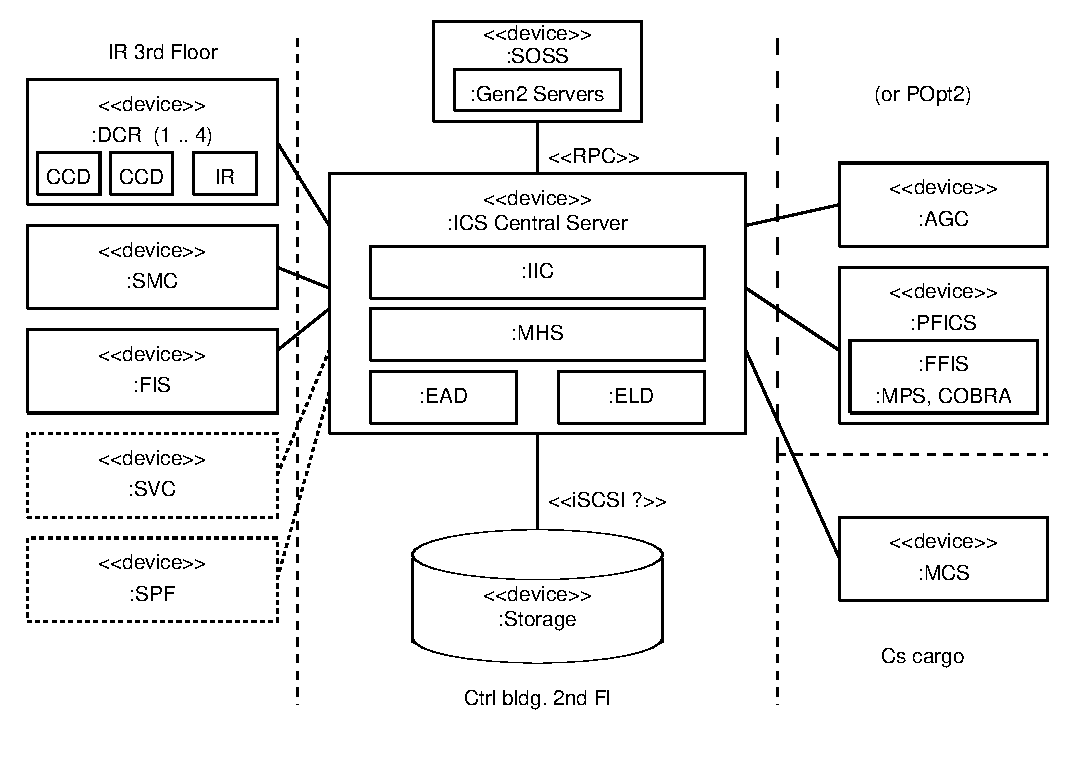
\includegraphics[scale=0.75]{deploy-diagram.eps}
  \end{center}
  \caption{Deployment diagram for entire PFS ICS}
  \label{fig:deploy-diagram}
\end{figure}


\subsection{Activities for one exposure}

For each exposure, following activities will be executed by ICS and its 
subsystems. 

\begin{itemize}
  \item (IF previous operation/activity was exposure, execute)
  \begin{itemize}
    \item IIC - SMC : Close shutter
    \item IIC - DCR : Readout CCD; Finalize IR detector data
  \end{itemize}
  \item (IF fiber arrangement is required, execute)
  \begin{itemize}
    \item IIC - SMC : Confirm shutter is closed
    \item IIC - FIS : Set blocking flag of FIS (allow control only from PFICS)
    \item IIC - PFICS : Release blocking flag of FFIS
    \item IIC - MCS : Set blocking flag of MCS (allow control only from PFICS)
    \item IIC - PFICS : Execute positioner movement, like
    \begin{itemize}
      \item PFICS - FIS : Confirm operation is allowed
      \item PFICS - FFIS : Confirm illuminator can be turned on
      \item PFICS - MCS : Confirm operation is allowed
      \item Execute loop sequence including MPS, MCS
      \item PFICS - FIS : Release blocking flag
      \item PFICS - MCS : Release blocking flag
    \end{itemize}
  \end{itemize}
  \item IIC - DCR : Confirm data were sent; (Or: Wait readout)
  \item IIC - FIS : Confirm illuminator is off; Set blocking flag of FIS (allow control only from IIC)
  \item IIC - PFICS/FFIS : Confirm FFIS is off; Set blocking flag of FFIS (no turn on)
  \item IIC - DCR : Execute reset (wipe) command
  \item IIC - SMC : Open shutter
  \item (Start exposure)
\end{itemize}



\section{Coordinate transform}

Even within PFS instrument, we have some independent coordinates for each 
subsystem. In this section, we will touch these coordinates and discuss 
necessary transformations among coordinates.
\footnote{Note: Text of this section is based on that of CoDR and PFI fiber 
alignment documents from JPL/CIT.}

\subsection{Definitions of Coordinates}

Definitions of possible coordinates and these relationships are defined 
as below.

\begin{description}
  \item[Sky coordinate]
    is the location (RA, Dec) of astronomical targets at some defined epoch
    (both standards like B1950.0, J2000.0, and at observation).
  \item[Delta sky coordinate] 
    is relative location (dRA, dDec) of astronomical targets in relative to 
    the selected pointing center position. 
  \item[Prime focus focal plane coordinate] 
    is a Cartesian coordinate system (x, y) located at the true focal plane
    of the POpt2 after the telescope and the WFC. 
    Origin shall be defined by the rotator axis of InR in POpt2.
    \footnote{Origin will not be defined by the optical axis of WFC, since 
    it is not easily measured and does not affect on a rotating center (except 
    for tolerance).}
  \item[Positioner bench coordinate] 
    is a Cartesian coordinate system at the plane of the fiber tips defined as 
    best fit to the fiducial fiber tips. Its origin is the nominal position 
    of the central fiducial fiber and is determined by fitting to the measured 
    positions of all fiducial fibers under "laboratory conditions", which 
    means a target is pointed at zenith considering an actual condition 
    mounted to the telescope, and any environmental condition (such as 
    temperature, relative humidity, barometric pressure) is stabilized 
    and well defined. 
  \item[COBRA coordinate] 
    is a set of ($\theta$, $\phi$) per each COBRA positioner, whose values are 
    defined by actual commanded positions. 
  \item[AGC coordinate] 
    is a Pixel coordinate system (x, y) on image detectors of each AGC.
  \item[MCS coordinate] 
    is a Pixel coordinate system (x, y) on an image detector of the MCS.
\end{description}




\subsection{Relationships between coordinates}

Relationships between coordinates are summarized as 
figure.~\ref{fig:coordinate-transform}, and each coordination transformation 
is described as followings. 
Also each bold faced is described after. 

\begin{figure}[htb]
  \begin{center}
    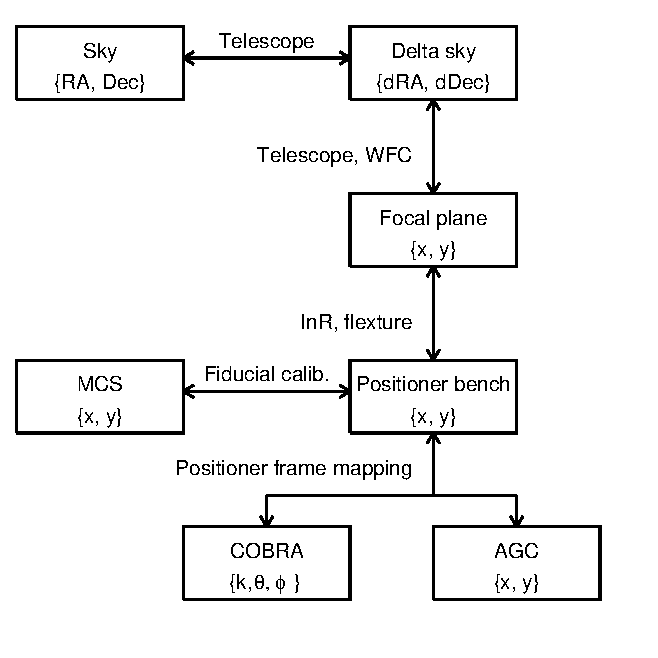
\includegraphics[scale=0.75]{coordinate.eps}
  \end{center}
  \caption{Relationship between coordinates and required transformations}
  \label{fig:coordinate-transform}
\end{figure}


\begin{description}
  \item[From Sky to Delta sky] 
    will be calculated by targeting software with a selected pointing center 
    position per exposure. 
    Since most of astronomical targets for PFS have small or no peculiar 
    motion, ICS will not be required to perform this transformation.
  \item[Delta sky to Focal plane]
    will be affected by the telescope, WFC, and ADC. 
    Transformation on {\bf Telescope and WFC distortion} shall be appried, 
    and {\bf ADC error} will remain without any correction. 
  \item[Focal plane to Positioner bench] 
    will be affected by the InR (Instrument Rotator) of POpt2 and {\bf flexture 
    of positioner frame and positioner bench}. Latter flexture will make two 
    coordinate (or its plane) different and is not correctable by coordinate 
    transformation. Excluding this effect, two coordinates should be on the 
    same plane and coordinate transformation will be described with two 
    parameters : rotation angle of InR and difference between two origins
    ({\bf Difference between InR rotator axis and positioner bench origin}). 
  \item[Positioner bench to MCS detector]
    is defined by four main parameters: 
    {\bf inverse viewing of WFC}; {\bf rotation axis offset, rotation angle, 
    and (optical) distance (magnification power) difference between 
    the positioner bench and MCS detector}. 
    Correction parameter of the {\bf inverse viewing of WFC} will be 
    measured by MSC itself using fixed fiducial fibers. 
    For others, rotation center difference, small rotation angle difference 
    \footnote{Note: since positioner bench (and fixed fiducial fiber 
    distribution) will be rotation symmetry by 60 degree, this difference 
    should be effectively smaller than this symmetry after corrected with 
    command value.}, and magnification will be also encoded by fixed fiducial 
    fibers. 
  \item[Positioner bench to COBRA positioners] 
    are on one identical plane and 
    will be transformed using {\bf a rotation centrer position and an origin 
    angle per each COBRA positioner}. 
    \footnote{COBRA positioners are tightly mounted on positioner bench, 
    their flexture and mounting accuracy shall be smaller than error budget.}
  \item[Positioner bench to AGC detector]
    are on one (virtually) identical plane and 
    will be transformed using {\bf a relative center position and an origin 
    angle per each AGC detector}. 
\end{description}

\subsubsection{Description of each correction}

Each correction will be organized as followings: 

\begin{description}
  \item[Telescope and WFC distortion] 
    will be measured and modeled by the HSC pipeline. 
    Since PFS has only AGC detectors on its focal plane, we are required to be 
    rely on the measurement and result of the HSC. 
  \item[Difference between InR rotator axis and positioner bench origin]
    will change on every exchange (remove and remount) between HSC and PFS 
    from POpt2. We are required to measure this offset just after every 
    remount onto POpt2. 
  \item[Inverse viewing of WFC]
    will be measured with using MCS and fixed fiducial fibers. This is not 
    directly related with the WFC distortion, but is a result through the same 
    corrector lens set. Therefore (highest) order required to be corrected 
    could be the same as one for the WFC distortion from sky to the focal 
    plane. 
  \item[Rotation axis offset, rotation angle, 
    and distance difference between 
    the positioner bench and MCS] 
    will be corrected using positions of fixed fiducial fibers imaged and 
    measured by a MCS detector. For every sequence, this will be re-measured 
    at the first shot. 
  \item[A rotation centrer position and an origin 
    angle per each COBRA positioner]
    will be measured during integration and test phase or commissioning phase, 
    and except for thermal expansion and flexture 
    this will not change until a maintenance of positioner bench, such as 
    fiber repairment (or exchange). 
  \item[A relative center position and an origin 
    angle per each AGC detector] 
    will be measured during integration and test phase or commissioning phase, 
    and except for thermal expansion and flexture 
    this will not change until a maintenance of positioner bench, such as 
    repairing or replacing. 
\end{description}

\subsubsection{Remaining and uncorrectable errors}

Also following errors would be included on some conditions or coordinate 
transformations and could not be corrected. 
These errors should be controlled and detected by an instrument design itself. 
\footnote{Note: this document is NOT to identify complete error sources.}

\begin{description}
  \item[Error from flexture of positioner frame and positioner bench] 
    are the difference in gravity induced translation and tilt by the 
    positioner frame compared to that by HSC dewar frame or WFC, and 
    flexture of positioner bench itself. 
  \item[ADC error]
    is uncorrected atmospheric refraction after ADC. 
    Considering PFS as wide wavelength ranged spectrograph, this error could 
    not be corrected by other correctors nor coordinate transformations. 
  \item[Thermal effects]
    will occur by changing environment temperature within POpt2. 
    For the telescope (outside of POpt2), this should be detected by an image 
    size on AGC and be corrected with moving hexapod of POpt2. 
  \item[Other flextures]
    will occur on every hardware, such as COBRA positioner itself 
    (gravitational condition changed), MCS internal and its fixed hard point 
    to the Cs interface, etc.
\end{description}

\subsection{Responsibilities on coordinate transformations}

Before this plan C, responsibilities on coordinate transformations are almost 
agreed, except for sharing common code modules for the distortion correction, 
\footnote{What part should be provided as common code modules is not yet 
agreed nor discussed among software team members. And also this kind of 
software development management should be discussed in separated from this 
plan.} 
and are summarized as table.~\ref{resp-coordtrans}. 
Since integration and test, commissioning, and engineering phases are 
separated from PFS science operation itself, this summary does not describe 
on data used during these coordinate transformations. 


\begin{table}[htb]
\caption{Summary of responsibilities on coordinate transformation}
\label{resp-coordtrans}
\begin{center}
\begin{tabular}{c|c|p{15em}}
  Transformation & Due & Remarks \\
  \hline
  Sky --- Delta sky & (not ICS)
    & This should be handled by targeting software \\
  \hline
  Delta sky --- Focal plane & IIC (IPMU)
    & To correct POpt2 hexapod, we will rely on SOSS (Gen2) system with using 
    images from AGC (so-called AGSequence in Gen2). \\
  \hline
  Focal plane --- Positioner bench & IIC (IPMU)
    & This includes monitoring and commanding to InR. \\
  \hline
  Positioner bench --- MCS & PFICS (CIT)
    & To measure 'center position' on MCS detector should be due to MCS. \\
  \hline
  Positioner bench --- COBRA & PFICS (CIT), MPS (JPL)
    & \\
  \hline
  Positioner bench --- AGC & AGC (ASIAA) or IIC (IPMU)
    & To measure 'center posision' on AGC detector should be due to AGC, 
    to convert from positioner bench coordination to actual command value 
    for A\&G or AG should be due to IIC. \\
\end{tabular}
\end{center}
\end{table}


\section{Terminology}

\begin{description}
  \item[AGC] Acquisition and Guidance camera system
  \item[API] Application Programming Interface
  \item[CUI] Character-based User Interface
  \item[DCR] Detector control and readout system
  \item[EMS] Environment monitoring systems
  \item[FIS] Fiducial fibers' back illuminating system
  \item[GUI] Graphical User Interface
  \item[ICS] Instrument Control Software
  \item[IIC] Instrument Interface and Controller
  \item[MCS] Metrology camera system
  \item[MHS] Messaging Hub Server
  \item[MLP] Mid-Level Processor of the Subaru telescope, which is 'sequencer' 
    of Mitsubishi Electric.
  \item[MPS] Movement Planning Software, which will command COBRA positioners.
  \item[PFICS] Prime Focus Instrument Control Software
  \item[PFS] Prime Focus Spectrograph for the Subaru telescope
  \item[SMC] Shutter mechanisms controller
  \item[SSF] Subaru Summit Facility, where entire PFS ICS will be delivered 
    to and will work at.
  \item[SVC] Slit viewing camera system
  \item[TCS] Telescope Control System of the Subaru telescope
\end{description}


\end{document}
